%% The following is a directive for TeXShop to indicate the main file
%%!TEX root = diss.tex

\chapter{A Problem Space of 3D Reconstruction}
\label{ch:3DRecon_ProbSpace}
We discussed the current landscape of 3D reconstruction in Chapter~\ref{ch:RelatedWork}. Previous research has solely focused on developing novel algorithms and softwares to tackle this problem. Thus, most research efforts have been devoted to improving algorithmic performance in terms of accuracy, completeness, computational efficiency, or relax restrictive assumptions so that they can be applied to more general situations. However, this approach, which we call an \textit{algorithm-centered} approach, faces two challenges: 1) it provides little to none insight into the conditions that allow a specific algorithm to work successfully; 2) it needs domain-specific knowledge to fine tune algorithm specific parameters to optimize the performance. This knowledge is either unknown or largely empirical, with each algorithm mapped roughly to a sub-volume in the \textit{problem space} that is poorly defined, thus requires vision knowledge to fully take advantage of these algorithms. In this thesis, \textit{problem space} is defined as a $N-$dimensional space which encompasses the material and shape of objects, and the axes of which consist of characteristic material and geometric attributes (called properties). The sub-volumn of the \textit{problem space} is called \textit{problem condition(s)}. We argue below that a well-defined \textit{problem space} is a critical part of designing an interface of 3D reconstruction, and should receive more research efforts.

% We are facing such challenges due to the following reasons: 1) the problem space is poorly defined, thus there is no way of describing the problem conditions in the first place; 2) compared to developing algorithmic novelties, it is generally a neglected research direction to study the problem conditions under which a specific algorithm works successfully.

We have established in Chapter~\ref{ch:RelatedWork} that most 3D vision algorithms target a limited set of problem conditions. They may work under one condition, but is highly likely to fail under others. Thus, they are unsuitable to reconstruct objects with a wide range of properties. Thus, it is crucial to have multiple algorithms, each registered to a distinct sub-volumn of the \textit{problem space} in order to design an interface for 3D reconstruction problem. To achieve this goal, we need to first propose key attributes of the problem as axes of this $N-$dimensional space, which lay the foundation of describing problem conditions in a consistent and rigorous manner. Next, we need to discover the relation between \textit{problem conditions} and algorithms so that we can know which algorithm performs well given a specific problem condition, which will be discussed in Chapter~\ref{ch:3DRecon_Mapping}. Recall that \textit{problem space} is an $N-$dimensional space, of which the axes are material and shape properties of objects. The reason we choose material and shape properties is that they can be visually and conceptually estimated, and are also widely used by typical 3D vision algorithms as reconstruction cues. With a well-defined \textit{problem space}, we are able to describe the characteristic properties of an object that are crucial for reconstruction. For instance, instead of describing a cup simply as a `cup', we can describe it as `a white, glossy porcelain cup with shallow strips on the surface'. The visual and geometric properties, represented by words such as `white', `glossy', and `shallow', are crucial in terms of determining which algorithm is able to perform well. We call it a \textit{problem-centered} approach. This approach transforms the 3D reconstruction problem from one requiring knowledge and expertise of specific algorithms in terms of \textit{how} to use them, to one requiring knowledge of problem conditions, which can be perceptually estimated or measurable. The advantage of the \textit{problem-centered} approach are as follows: 1) the properties can be universally used by most objects, without the need of algorithm-specific parameters; 2) the properties of the \textit{problem space} can be visually or conceptually estimated. Thus, there is no need to understand the meanings of algorithm parameters, \ie no vision knowledge required.

% Note we have specifically focused on the material and geometric properties of the objects, as they are the cues used by many vision algorithms, and also the key components of the problem space. It then becomes possible to evaluate the performance of algorithms under this well-defined conditions, which generates a one-to-one relation between problem space and algorithms. 

In this chapter, we first propose a well-defined problem space consisting of visual and geometric properties of objects in Section~\ref{sec:prob_space}. Since the problem space is generally too vast to tackle, we state addition assumptions and underlying rationales to limit the scope of problem space in Section~\ref{sec:prob_space}. Finally, we propose four main problem conditions that we are interested in investigating in this thesis.

% First, we need to have a better understanding of the problem space. In this thesis, what we mean problem space is the volume of reflectance and shape variations that objects occupy. We first describe the visual and geometric properties that constitute this problem space, then we provide further discussions regarding additional assumptions and underlying rationales to further narrow the problem space, and propose the 

% Developers started to come up with applications and working scenarios that are suitable for the developed algorithms. This approach to problem solving leads to so many examples of excellent technology, yet poor applications. The scientific approach to problem solving starts with defining the problem of interest. Without a formal understanding of the problem space, any efforts towards solving the problem have the risk of getting stuck in a deadend or diverging into a totally different and irrelevant direction and ending up with an undesired solution. The same logic applies to the research on 3D reconstruction. Thus, this chapter sets out to gives a comprehensive definition to the field of 3D reconstruction, and states additional assumptions to narrow the problem space so that it can be tackle within this thesis.

\section{Problem space}
\label{sec:prob_space}
We first give an overview of problem space, which consists of visual and geometric properties of real-world objects, as shown in Figure~\ref{fig:obj_class}. These properties can be conceptualized as dimensions/axes of the 3D reconstruction problem space. This approach allows us to think of algorithms pointing to volumes within an $n-$dimensional problem space. Existing algorithms can be incorporated into the interface by evaluating the algorithmic performance within the problem space, as shown in Figure~\ref{fig:embed_algo}. However, by no means are the presented problem space complete. There are many other properties not included that are commonely seen in the real world. For instance, properties such as metalness, emission, occlusion, discontinuity, among others, are not considered. However, the listed set of properties are broad enough to encompass a wide range of real-world objects. To help easy identification of a specific problem condition, we propose the following labels to differentiate object classes, as shown in Table~\ref{tab:prop_label}.
\begin{figure}[!htbp]
\centering
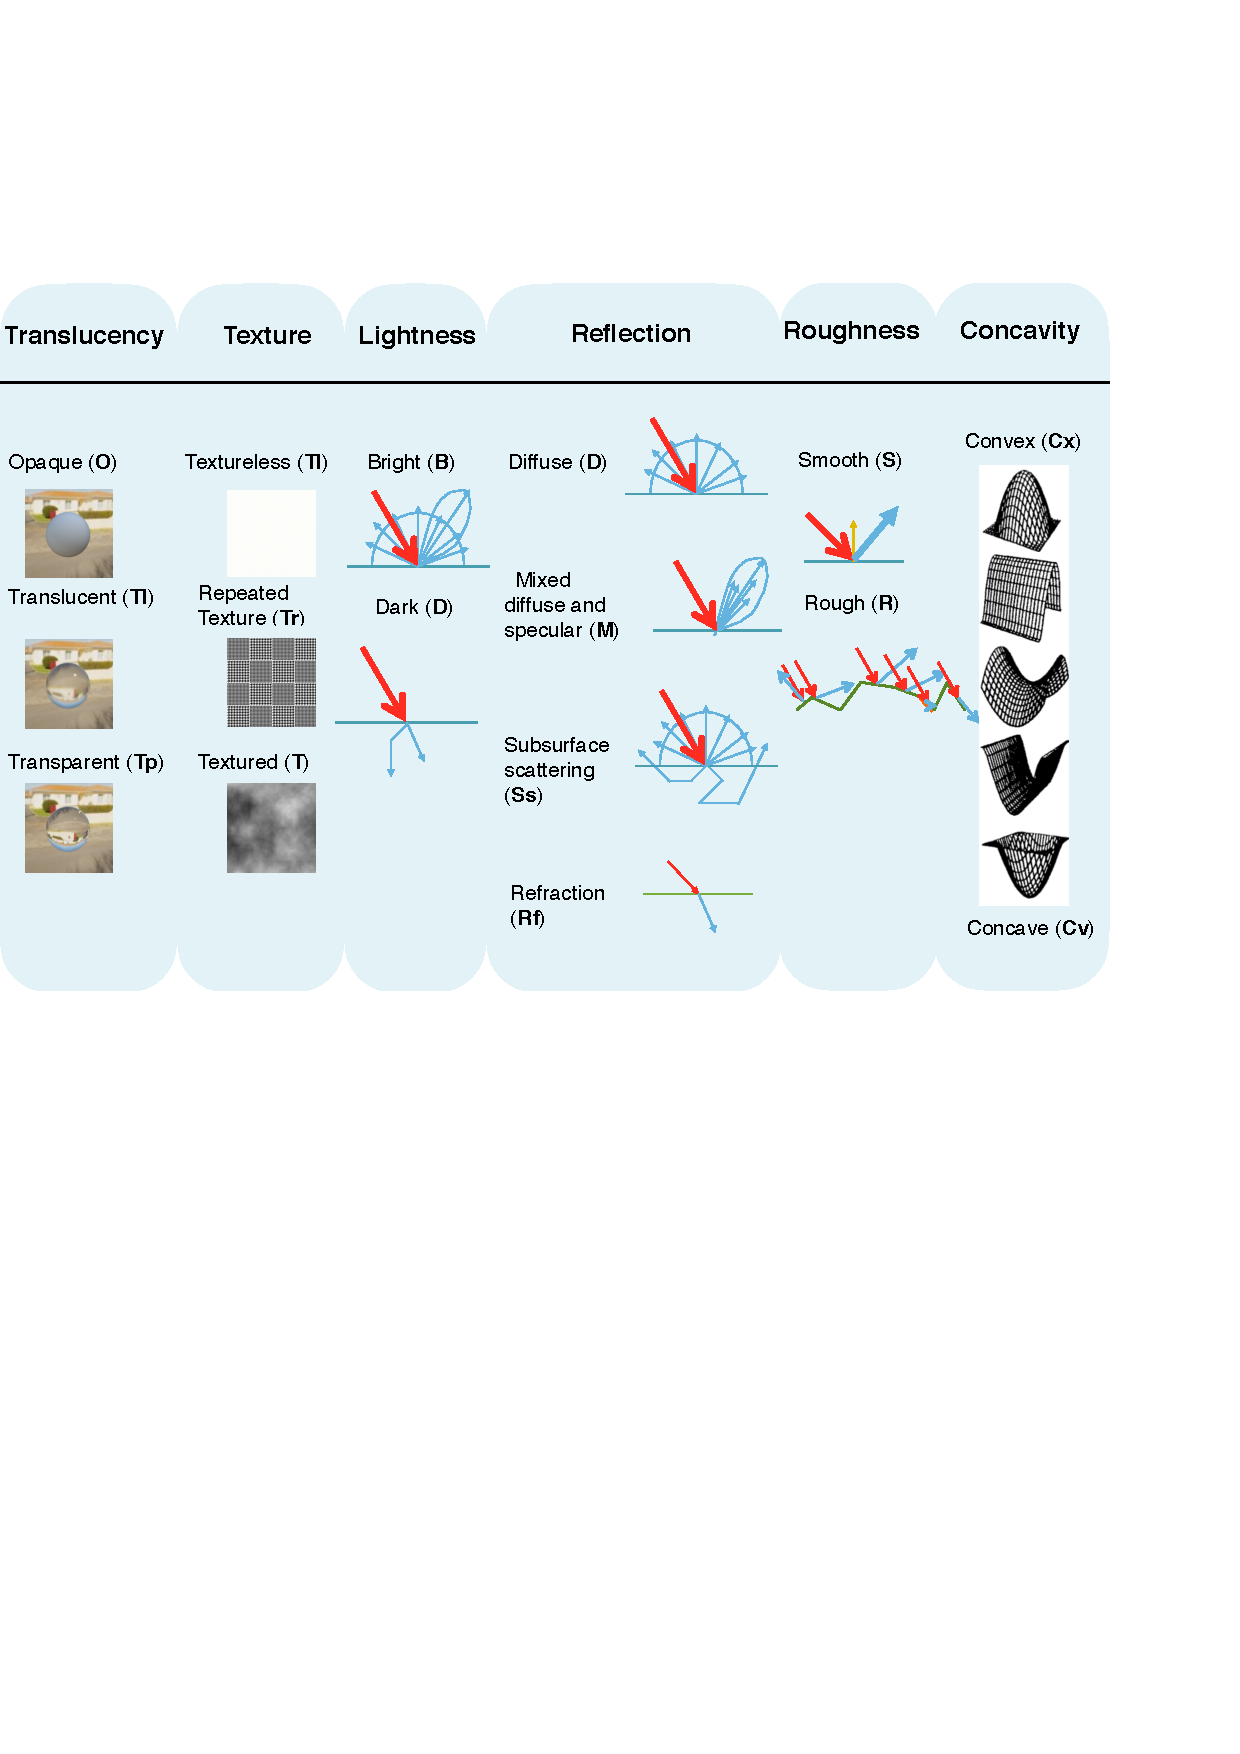
\includegraphics[width=\textwidth]{prob_space/obj_class}\\
\caption{A list of properties for problem space.}
\label{fig:obj_class}
\end{figure}

%\begin{table}[!htbp]
%\centering
%\begin{tabular}{l | ll}
%\toprule
%Property name & Property value & Property label \\
%\midrule
%\multirow{3}{*}{Translucency} & Opaque & \textbf{O} \\
%							  & Translucent & \textbf{Tl} \\
%							  & Transparent & \textbf{Tp} \\ \cline{2-3}
%\multirow{3}{*}{Texture} & Textured & \textbf{T} \\
%						 & Repeated textured & \textbf{Tr} \\
%						 & Textureless & \textbf{Tl} \\ \cline{2-3}
%\multirow{2}{*}{Lightness} & Bright & \textbf{B} \\
%						   & Dark 	& \textbf{D} \\ \cline{2-3}
%\multirow{5}{*}{Reflection} & Specular model & \textbf{S} \\
%							& Diffuse model  & \textbf{D} \\
%							& Mixed model	 & \textbf{M} \\
%							& Sub-surface scattering & \textbf{Ss} \\
%							& Refraction 	 & \textbf{Rf} \\ \cline{2-3}
%\multirow{2}{*}{Roughness} & Smooth & \textbf{S} \\
%						   & Rough 	& \textbf{R} \\ \cline{2-3}
%\multirow{2}{*}{Concavity} & Convex  & \textbf{Cx} \\
%						   & Concave & \textbf{Cv} \\
%\bottomrule
%\end{tabular}
%\caption{Labels of properties}
%\label{tab:prop_label}
%\end{table}

\section{Assumptions}
\label{sec:assumptions}
Though 3D reconstruction of opaque surfaces with Lambertian reflectance has been a well studies problem, specular, translucent, transparent, and refractive scenes still pose challenging problems for acquisition systems~\cite{ihrke2010transparent}. ~\citeauthor{ihrke2010transparent} conducted a comprehensive review on acquisition approaches for transparent and specular surfaces, and concluded that though different classes of techniques have been developed to deal with these problems and good reconstruction results can be achieved with current state-of-the-art techniques. However, the proposed approaches are still highly specialized and targeted at a very specific object class~\cite{ihrke2010transparant}. Thus, the limits of existing techniques demands that only a subset of the problem space can be explored. Further, it makes it more feasible as a proof of concept demonstration. Therefore, we make the following assumptions to the problem:

\subsubsection{Simplified light interaction model}
We assume \textbf{local interaction model}, \ie global light transport such as transmission, refraction, cast shadow, inter-reflection, metalic are not considered. The rationale behind our choice is that most techniques that have been developed over the past few decades mainly tackle object with an opaque, diffuse or mixed surface. For specular, refractive, and translucent or transparent objects, only very specialized algorithms are applicable for reconstruction~\cite{ihrke2010transparent}. This is a widely used and accepted model in varied areas of computer vision, including shape from stereo, shading, and so on. As more algorithms become available to tackle these types of objects, they can be embedded to the interface using the same approach will be discussed in Chapter~\ref{ch:3DRecon_Mapping}, as shown in Figure~\ref{fig:embed_algo}.
\begin{figure*}[!htbp]
\centering
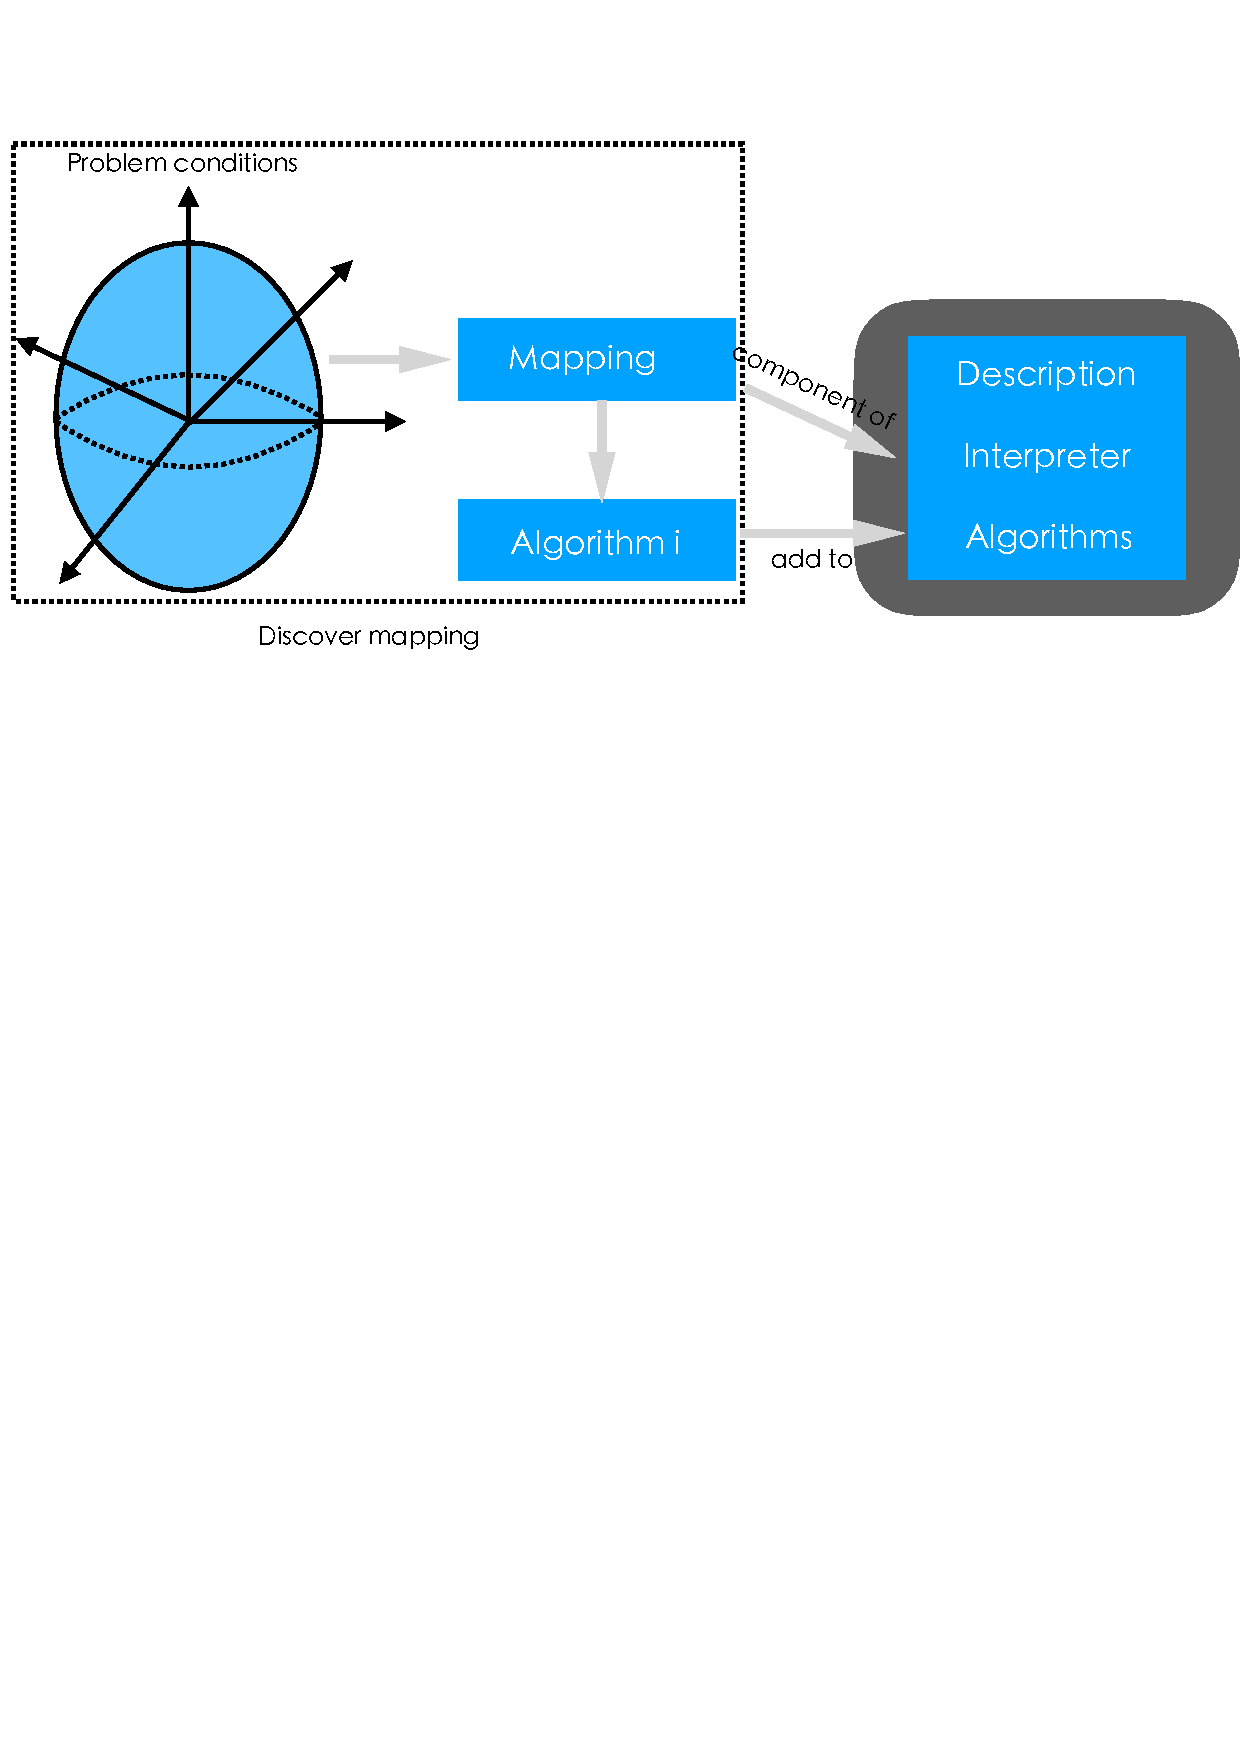
\includegraphics[width=0.8\textwidth]{img/prob_space/embed_algo.pdf}
\caption{Embed algorithms into the interface.}
\label{fig:embed_algo}
\end{figure*}

\subsubsection{Simplified reflectance model}
Since the majority of reconstruciton techniques rely on observing light reflected off a surface, surfaces exhibit significant effect of global light tranport present a huge challenge to the reconstruction problem. Surface exhibits global light transport, including \textit{specular}, \textit{transmission}, \textit{sub-surface scattering}, \textit{inter-reflection}, \textit{self-shadow}, and etc would break the assumptions made by most generic 3D reconstruction algorithms. Thus the global light transport are ignored, and the reflection properties of consideration are \textit{albedo}, \ie the ratio of reflected light w.r.t the received light, and \textit{specularity}, \ie the amount of specular reflection. A more comprehensive model should be constructed based on our work to incorporate more complex phenomena to be more comprehensive.

\subsubsection{Simplified geometric model}
It's a challenging task to model geometry using mathematical descriptions. For geometric primitives such as cube, sphere, or cone, etc, it's possible to describe the shape using concise descriptions. However, the task becomes prohibitive when it comes to shapes with varied characteristics. Furthermore it becomes more ambiguous when natural language is employed. Thus we only consider the microscopic roughness of the surface, which has a direct relation with the reflection. Other prominent geometric properties such as \textit{concavity}, which affects self-shadow, inter-reflection, \textit{depth-discontinuity}, which affects the depth estimation, are ignored.

\subsubsection{High surface albedo}
Existing 3D vision techniques requires distinct cues for reconstruction, be it texture, intensity variation, focus change, and so on. This information will become much noisier and less effective on darker surfaces. Surfaces with low albedo will make many candidate algorithms ineffective, including most active techniques. In this thesis, dark surfaces could be challenging for all the underlying algorithms used in this thesis. This is fine in term of designing an interface since there is no need for all underlying algorithms to work well. However, from a demonstrative standpoint, this would fail to demonstrate the performance of interpreter since it would most likely select the baseline method. To avoid such situations, we decided to use objects with bright surfaces so that reconstruction cues to easier to detect.

\subsubsection{Setup of capturing system}
The configuration of capturing system determines the selection of algorithm in a variety of ways. The capturing device determines what type of data is captured, which could be RGB images, or range data depending on whether a camera of laser scanner is used. The lighting condition determines if a passive or active method is selected since active methods need controlled lighting. The number of vantage points determines if data from different viewpoints or under different illuminations are needed. In short, variations in the capturing systems can greatly impact which algorithm is effective, or the performance of algorithms. This significantly increases the complication of the problem. Thus, we decide to use a fixed capturing system throughout the thesis. However, note that the results obtained under this capturing system might not be applied to data captured using a different capturing system. However, the approach would not be affected by the hardware setup.

% \subsection{Four problem conditions}
% \label{sec:prob_cond}
Built upon the previously defined problem space, and additional assumptions, we define four classes of problem conditions that will be investigated in depth, as shown in Figure~\ref{fig:prob_cond}. We will demonstrate that it is achievable to design a descritpion-based interface that hides algorithm details and return solutions without knowing the underlying algorithms using objects that satisfy these conditions.
\begin{figure*}[!htbp]
\centering
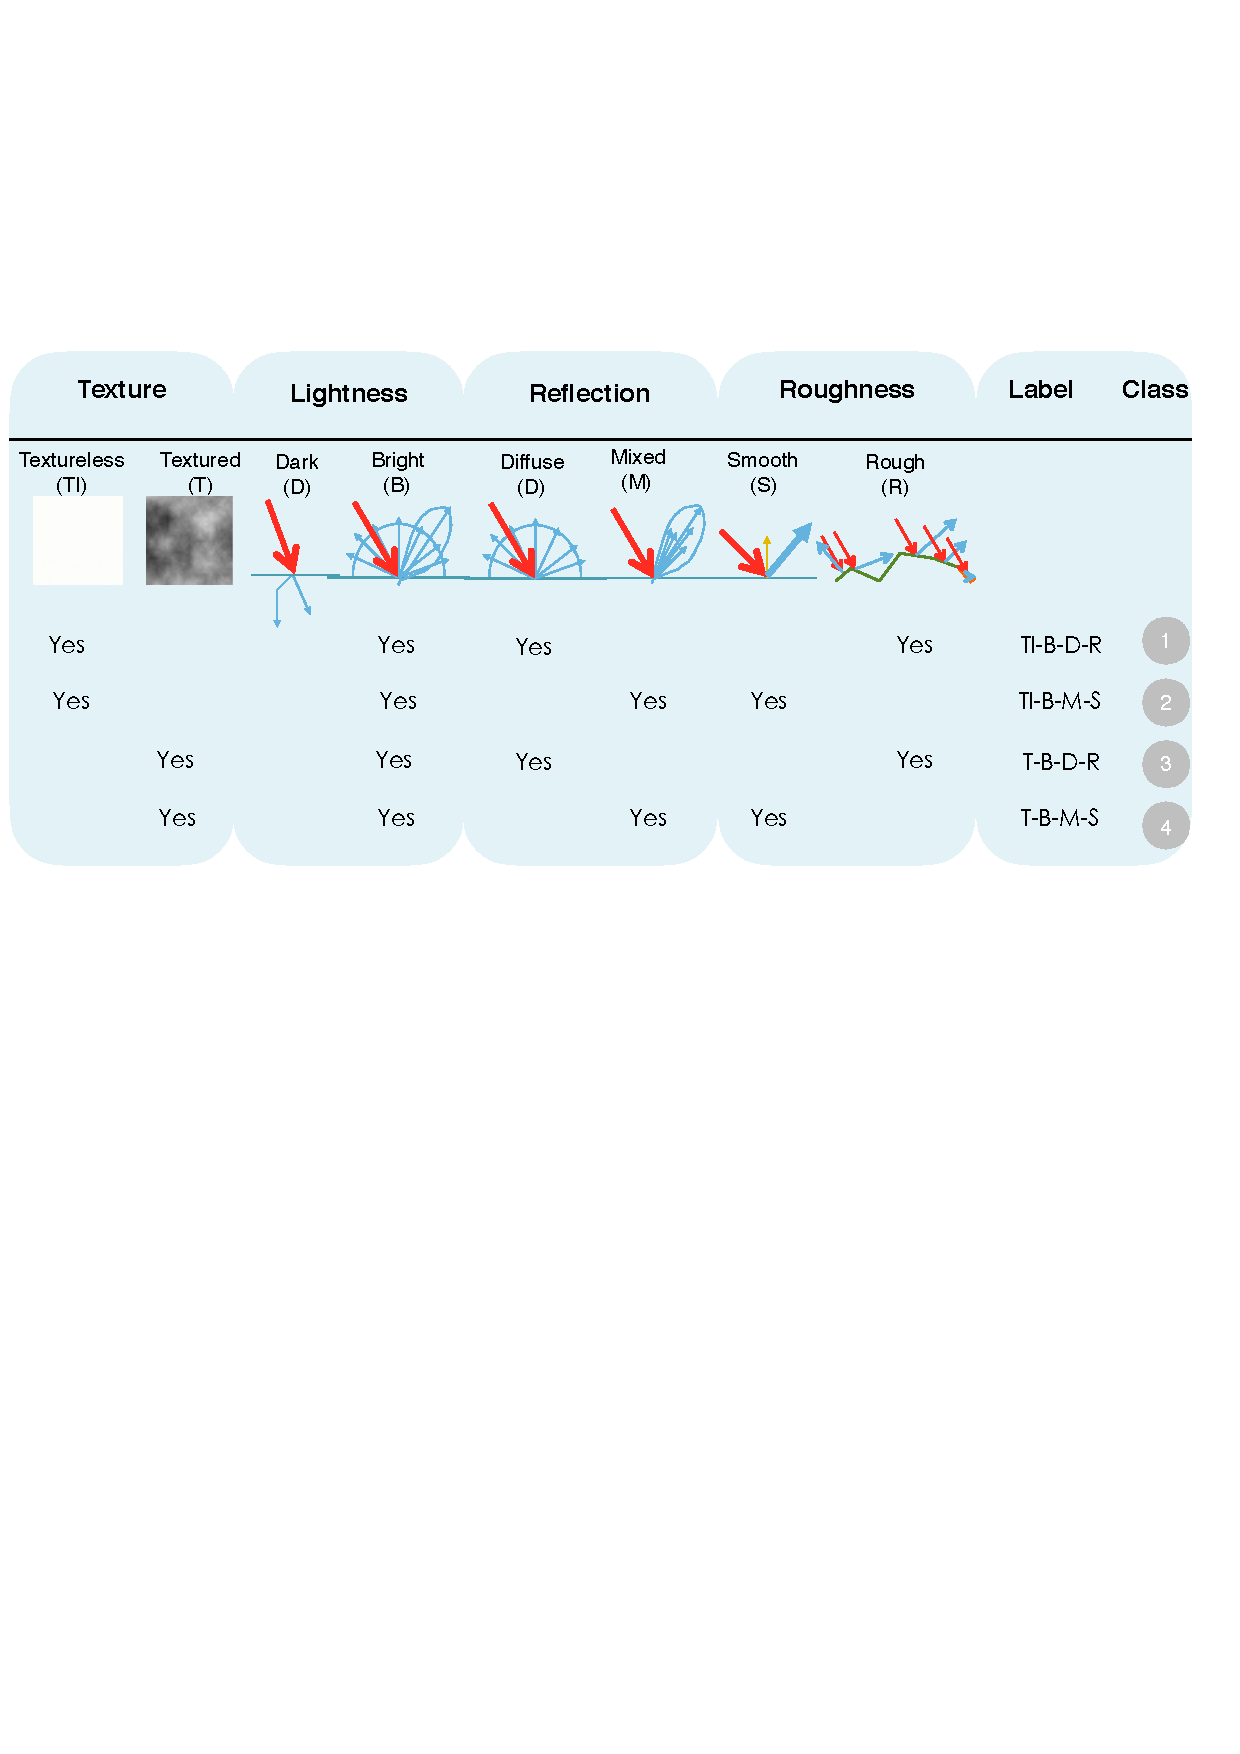
\includegraphics[width=\textwidth]{prob_space/prob_cond}
\caption{Four problem conditions selected based on the definition of problem space and additional assumptions. The description-based interface will be evaluated using objects satisfying these conditions.}
\label{fig:prob_cond}
\end{figure*}

\subsection{Discussion and Conclusions}
Most vision research has been devoted to developing algorithmic novelties and improving performance. However, the conditions under which an algorithm works reliably is often a neglected subject. However, this is a crucial part to design a 3D reconstruction interface. Since no single algorithm can work reliably under a wide range of conditions, it is required to have multiple algorithms, each covering a distinct or partially overlapping conditions. The problem then becomes under which condition can an algorithm work successfully. To answer this question, we first need to define the problem space and problem conditions. Otherwise, it is a poorly-defined task to describe the problem condition of an object.

We first proposed a well-defined problem space, which is an $N-$dimensional space, the axes of which are reflective and geometric properties of objects. The problem condition(s) is then defined as a sub-volumn within the problem space. Since existing 3D vision algorithms can only deal with certain classes of objects, we further proposed assumptions to limit the problem space to a more feasible range. Further, to implement a proof of concept interpreter for demonstrative purpose, we choose four problem conditions to demonstrate the proposed interpreter.

Since this thesis studies a sub-space of the entire problem space, a natural question is whether this approach extends to a broader space when incorporating properties that have been left out, such as refraction, sub-surface scattering, and so on. This is a challenging task, and depends on two aspects: 1) robust techniques that work successfully under these conditions have been developed; 2) there is a way to describe the corresponding properties. The goal of this thesis is to demonstrate whether it is possible for the proof of concept interpreter to find a reliable algorithm given a description of problem condition. Thus, this is left as a future research direction.
